\documentclass{article}
\usepackage[export]{adjustbox}
\usepackage{graphicx}
\usepackage{fancyvrb}


\title{Reporte Actividad 5}
\author{Andr\'es Rodr\'iguez}
\date{}


\begin{document}

\maketitle

\graphicspath{ {Imagenes/} }


\section{Introducci\'on}\

Se realiza un programa que ejecuta una simulaci\'on del movimiento de un proyectil especificando la velocidad inicial y el \'angulo inicial al que es lanzado. Lo resultados se guardan en la ejecuci\'on del programa en un archivo .dat, que posteriormente se utiliza para graficar las trayectorias. Y se muestran en pantalla los resultados te\'oricos del valor de tiempo de vuelo, altura m\'axima y alcance m\'aximo del proyectil por medio de las siguientes ecuaciones:\\ \\
Tiempo de vuelo
$$t=\frac{2 v_0 sin(\theta)}{g}$$
\ Altura m\'axima
$$h=\frac{v_0^2 sin^2(\theta)}{2g}$$
\ Alcance m\'aximo
$$d=\frac{v_0^2}{g} sin(2\theta)$$


\section{Resultados}\

Se muestra una imagen de pantalla de la ejecuci\'on del programa para realizar los c\'alculos con sus respectivos angulos iniciales. La velocidad inicial en cada uno de ellos se tom\'o como 150.

\begin{itemize}

\item 90 grados\\
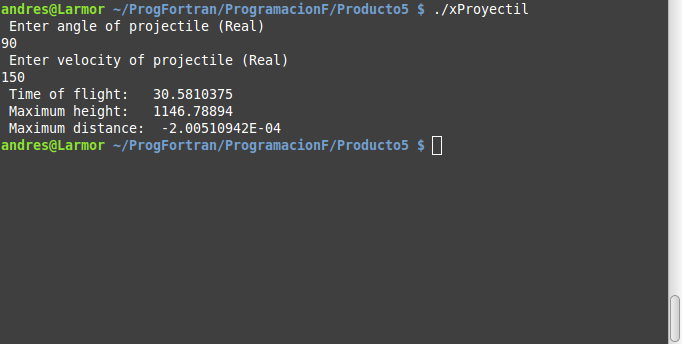
\includegraphics[scale=.5]{90}
\item 60 grados\\
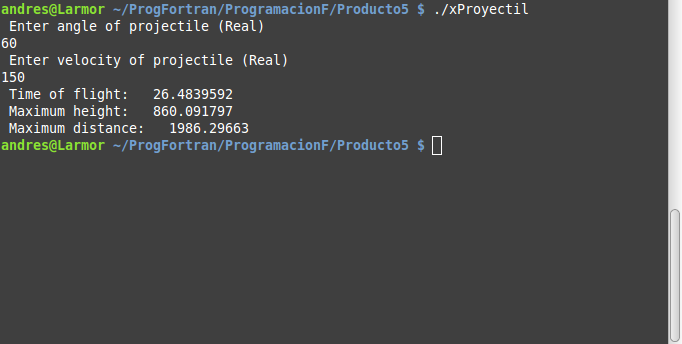
\includegraphics[scale=.5]{60}
\item 45 grados\\
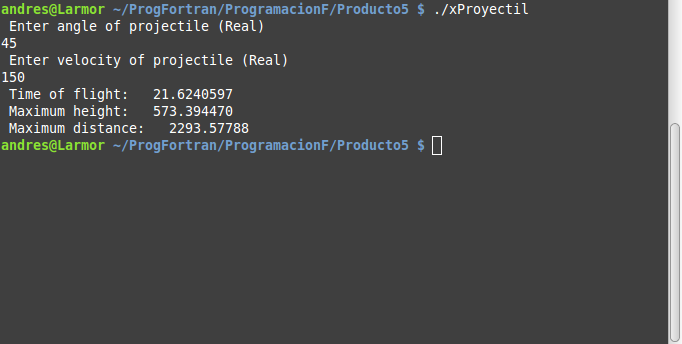
\includegraphics[scale=.5]{45}
\item 30 grados\\
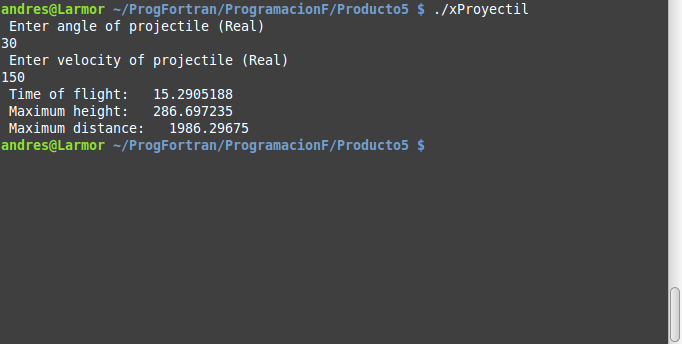
\includegraphics[scale=.5]{30}
\item 0 grados\\
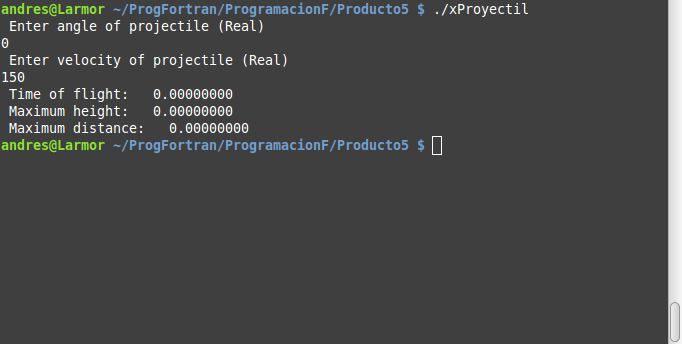
\includegraphics[scale=.5]{0}
\item Gr\'afica de los datos obtenidos\\ \\
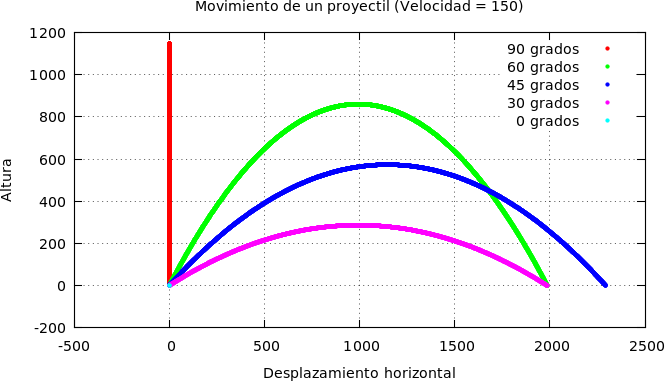
\includegraphics[scale=.6]{proyectiles}


\end{itemize}


\section{C\'odigo}

C\'odigo Fortran:\\
\begin{Verbatim}[frame=single]

 program projectile_plot  
       implicit none  
       !Defining constants:  
       real, parameter :: pi = 4.0*atan(1.0) 
       real :: u, a, t, a_grados  , Tt, H, R
       real, parameter :: g = 9.81  
       real:: x,y  
          integer :: i 

       !where g is gravity, pi is "pi"   
       !u is object's initial velocity   
       !a is object's initial angle   
       !t is time during the simulation   
       !x and y are arrays with 150 rows   
       !Seek user input   
       write(*,*) 'Enter angle of projectile (Real)'   
       read *, a_grados   
       write(*,*) 'Enter velocity of projectile (Real)'   
       read *, u   
       !Convert angle to radians   
       a = a_grados*pi/180.0   
      
       i=0

       open(1, file='proj.dat')   
      

       do  while ( y >= 0 )
            !displacement of object in x and y direction   
            t = (float(i)*0.01)   
            x = u*cos(a)*t   
            y = u*sin(a)*t - 0.5*g*t*t   
            !write output in file "proj.dat" for plotting   
            write(1,*) x, y  
            !kill the loop when the object hits the ground    
            i = i + 1
       end do   
       close(1)   
       !close file
       
Tt = 2*u*sin(a)/g
H = u*u*sin(a)*sin(a)/(2*g)
R = u*u*sin(2*a)/g

       write(*,*) 'Time of flight:', Tt
       write(*,*) 'Maximum height:', H
       write(*,*) 'Maximum distance:', R

   
  end program projectile_plot 



\end{Verbatim}


\end{document}